% natbib guide (https://gking.harvard.edu/files/natnotes2.pdf)
% \citet     #textual citations, print the abbreviated author list
% \citet*    #textual citations, print the full author list
% \citep     #parenthetical citations, print the abbreviated author list
% \citep*    #parenthetical citations, print the full author list
% \citealt    #the same as \citet but without any parentheses.
% \citealp    #the same as \citep but without any parentheses. 
% \citeauthor{ale91}         #Alex et al.
% \citeauthor*{ale91}        #Alex, Mathew, and Ravi
% \citeyear{ale91}           #1991 
% \citeyearpar{ale91}        #(1991)

\documentclass[english, xcolor=dvipsnames, aspectratio=169]{beamer}

% Text encoding
\usepackage[english]{babel}

% Justify text (package and function)
% \apptocmd{command}{code}{success}{failure}
\usepackage{ragged2e}
\apptocmd{\frame}{}{\justifying}{} 
% Justify text in \item
\newcommand{\itemj}{\item \justifying}

% If...else package
\usepackage{ifthen}

% Package to set transparent background image
\usepackage{tikz}

% Include image package
\usepackage{graphicx}
% Set default path for images
\graphicspath{ {./imgs/} }
% Set figure number when included
\setbeamertemplate{caption}[numbered]

% Bibliography packages
\usepackage[sort, round]{natbib}
\bibliographystyle{plainnat}

% Define colors variables
\definecolor{darkblue}{rgb}{0.12, 0.139, 0.164} % primary color
\definecolor{grey}{rgb}{0.3686, 0.5255, 0.6235} % secondary color

% Set theme palette colors
\setbeamercolor{palette primary}{bg=darkblue,fg=white}
\setbeamercolor{palette secondary}{bg=darkblue,fg=white}
\setbeamercolor{palette tertiary}{bg=darkblue,fg=white}
\setbeamercolor{palette quaternary}{bg=darkblue,fg=white}
% strucure means itemize, enumerate, etc
\setbeamercolor{structure}{fg=darkblue} 

% Set bibliography colors
\setbeamercolor{bibliography item}{fg=darkblue}
\setbeamercolor{bibliography entry author}{fg=black}
\setbeamercolor{bibliography entry title}{fg=black}
\setbeamercolor{bibliography entry location}{fg=black}
\setbeamercolor{bibliography entry note}{fg=black}
% Replaces book icon in bibliography with enumeration
\setbeamertemplate{bibliography item}{[\theenumiv]}

% Table of contents style
% \setbeamertemplate{section in toc}[sections numbered]
% \setbeamertemplate{subsection in toc}[subsections numbered]
\setbeamertemplate{section in toc}[circle]
\setbeamertemplate{subsection in toc}[ball unnumbered]

% Header with navigation bar
\setbeamertemplate{headline}
{
    \leavevmode
    \hbox{
    \begin{beamercolorbox}[wd=\paperwidth,ht=2.5ex,dp=1.125ex]{palette quaternary}
    \insertsectionnavigationhorizontal{\paperwidth}{}{\hskip0pt plus1filll}
    \end{beamercolorbox} 
    }
}
% Footer with custom caption

\setbeamertemplate{footline}
{
    \leavevmode
    \hbox{
    \begin{beamercolorbox}[wd=.33\paperwidth,ht=2.6ex,dp=1ex,center]{palette quaternary}
    \usebeamerfont{author in head/foot}\insertshortauthor\hspace*{1ex}
    \end{beamercolorbox}
    \begin{beamercolorbox}[wd=.33\paperwidth,ht=2.6ex,dp=1ex,center]{palette quaternary}
    \usebeamerfont{institute in head/foot}\insertshortinstitute
    \end{beamercolorbox}
    \begin{beamercolorbox}[wd=.33\paperwidth,ht=2.6ex,dp=1ex,center]{palette quaternary}
    \insertframenumber{} / \inserttotalframenumber
    \end{beamercolorbox}}
    \vskip0pt
    
}

% Global Background must be put in preamble
\usebackgroundtemplate
{
    \tikz\node{
\includegraphics[height=\paperheight, width=\paperwidth]{background.pdf}};
}

% One line command to print table of contents - two parameters for modes
\newcommand{\customToC}[2]
{
    \begin{frame}{Overview}
    \tableofcontents[#1,#2]
    \end{frame}
}

% Command to plot centered figure
% Parameters: #1=image name, #2=caption 
\newcommand{\includefigure}[2]
{
    \begin{figure}[h]
    \caption{#2}
    \centering
    \includegraphics[width=0.5\textwidth]{#1}
    \end{figure}
}

% Command to set section name as variable (\renewcommand to update)
\newcommand{\sectiontitle}{}
% Command to set subsection name as variable (\renewcommand to update)
\newcommand{\subsectiontitle}{}


% Title page
\title{The eNanoMapper Ontology}
\subtitle{Harnessing ontologies to enable data integration for nanomaterial risk assessment}
\author{Javier Millán Acosta}
\institute{BiGCaT - Maastricht University}
% Date
\day=19\relax
\month=09\relax
\year=2022\relax

\begin{document}

\frame{\titlepage}

% Complete table of contents (ToC)
% \customToC{hideallsubsections}{}
\customToC{}{}

% Section name and highlighted ToC
\renewcommand{\sectiontitle}{Introduction}
\section{\sectiontitle}
\customToC{currentsection,hideothersubsections}{}

% Section name and highlighted ToC
\renewcommand{\subsectiontitle}{eNanoMapper}
\subsection{\subsectiontitle}
\begin{frame}{\subsectiontitle}
    \emph{\textit{eNanoMapper aims to address data and model interoperability challenges for toxicological data management for ENMs. This ontology is an application ontology targeting the full domain of nanomaterial safety assessment. It re-uses several other ontologies.}}
    % Include figure with caption
    \includefigure{eNanoMapper_LOGO.png}{The eNanoMapper logo}
\end{frame}
\begin{frame}{\subsectiontitle}
Engineered nanomaterials are (...)
\end{frame}

% 
\renewcommand{\subsectiontitle}{What is an ontology?}
\begin{frame}{\subsectiontitle}
    \begin{itemize}
        \item A means to capture things \citet{source}
        \item It consists of a set of statements (axioms) each of which is true in the situation it is applied to. \citet{source}
    \end{itemize}
\end{frame}

% 
\begin{frame}{\subsectiontitle}
    \begin{itemize}
        \item Classes
        \item Individuals
        \item ...
    \end{itemize}
\end{frame}

% 

\begin{frame}{\subsectiontitle}
    \begin{itemize}
        \item \textbf{Foundation ontologies}: they provide the most abstract or general classes, i.e., the top-level classes we see in a hierarchy view of our ontology.
        \item \textbf{Application ontologies}:
        \item \textbf{Domain ontologies}
    \end{itemize}
\end{frame}

% 
\begin{frame}{\subsectiontitle}
    \begin{itemize}
        \item \textbf{An ontology is stored in a text file}
        \item \textbf{An ontology is a }
        \item ...
    \end{itemize}
\end{frame}

% 
\subsection{\subsectiontitle}
\begin{frame}{\subsectiontitle}
    \begin{itemize}
        \item Foundation ontologies
        \item OBO ontologies
        \item Chebi
        \item GO
    \end{itemize}
\end{frame}

% 
\renewcommand{\subsectiontitle}{What does an ontology look like? (cont)}

\begin{frame}{\subsectiontitle}
    \begin{figure}[ht]
        \begin{minipage}[b]{0.35\linewidth}
            \centering
            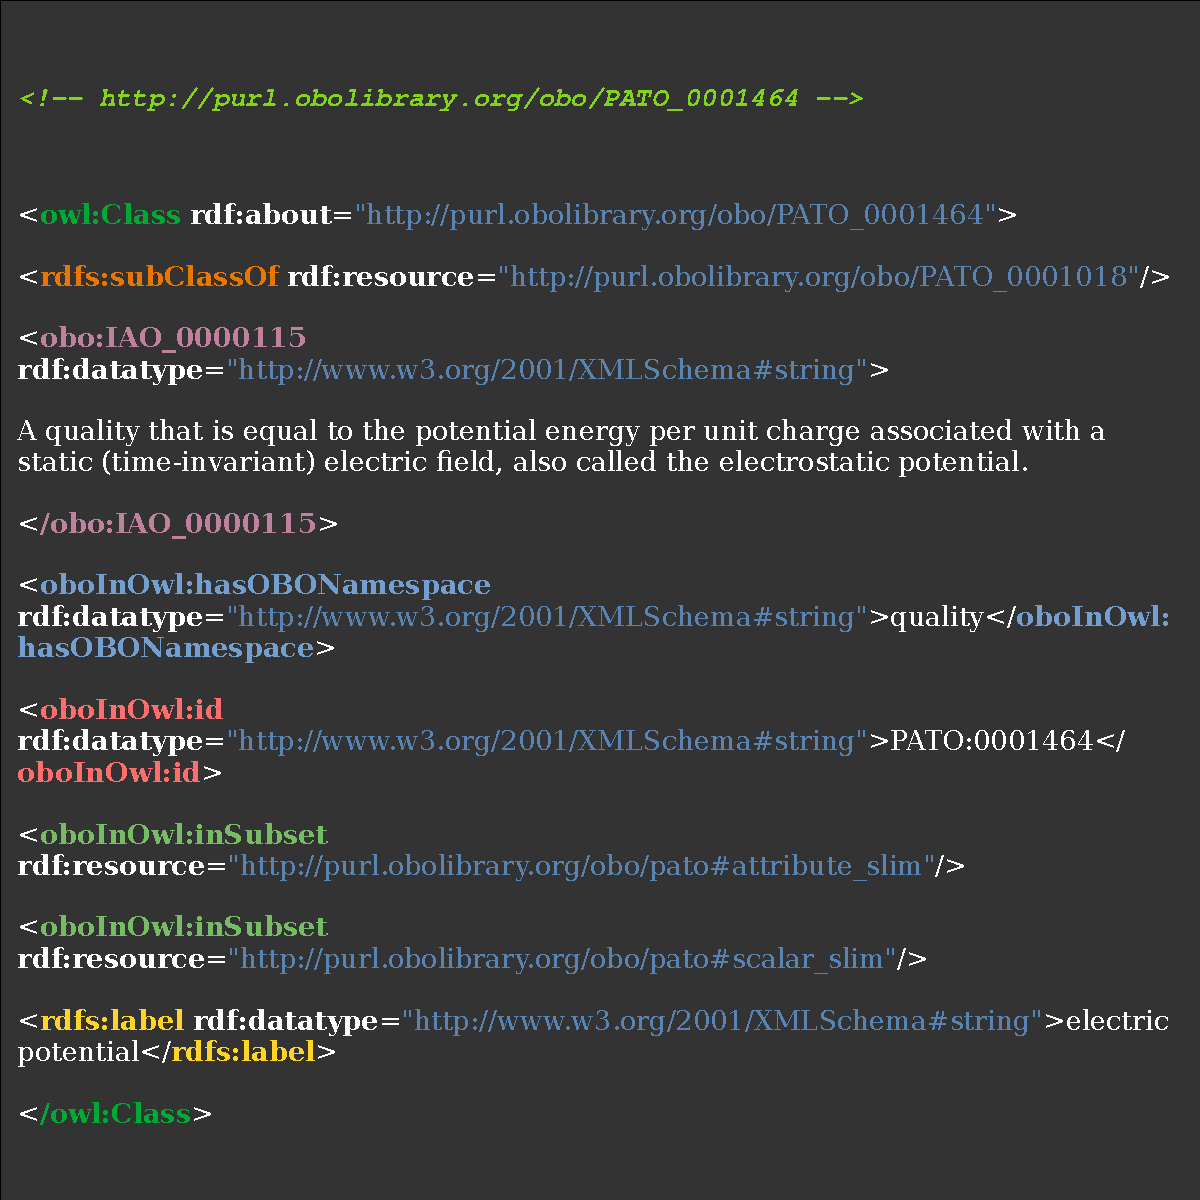
\includegraphics[width=\textwidth]{owltext.pdf}
            \caption{A class in an ontology text file}
            \label{fig:cifar10}
        \end{minipage}
        \hspace{0.5cm}
        \begin{minipage}[b]{0.35\linewidth}
            \centering
            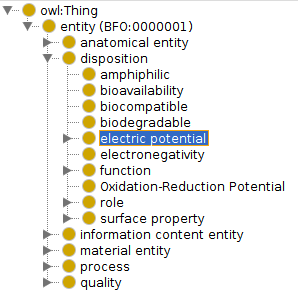
\includegraphics[width=\textwidth]{classhierarchy.png}
            \caption{A class in the hierarchy view of an ontology}
            \label{fig:cifar100}
        \end{minipage}
    \end{figure}
\end{frame}


% Section name and highlighted ToC
\renewcommand{\sectiontitle}{Current state of the eNanoMapper Ontology}
\section{\sectiontitle}
\customToC{currentsection,hideothersubsections}{}


% 
\renewcommand{\subsectiontitle}{Development and QC}
\subsection{\subsectiontitle}

\begin{frame}{\subsectiontitle}
    Pointers about this...
    
\end{frame}

% 
\renewcommand{\subsectiontitle}{Uses of the eNM ontology}
\subsection{\subsectiontitle}

\begin{frame}{\subsectiontitle}
    Pointers about this...
    
\end{frame}


%
\renewcommand{\sectiontitle}{Future plans and challenges}
\section{\sectiontitle}
\customToC{currentsection,hideothersubsections}{}

% 
\renewcommand{\subsectiontitle}{What is still needed}
\subsection{\subsectiontitle}

\begin{frame}{\subsectiontitle}
...
\end{frame}

% 
\renewcommand{\subsectiontitle}{Migrating the ontology development?}
\subsection{\subsectiontitle}
\begin{frame}{\subsectiontitle}
... ODK for automation, standadisation, interoperability... is it convenient for enm?
\end{frame}



% Import bibliography from file sample.bib
\begin{frame}[t, allowframebreaks]
\frametitle{References}
\bibliography{sample}
\end{frame}

\end{document}